\subsection{Descripción del funcionamiento}
Nuestra propuesta para solventar algunas desventajas de los sistemas de energía renovable (especialmente la solar) es crear un sistema autónomo e inteligente que, a través de un sistema off-grid, sea capaz de acoplar y desacoplar la casa de la red eléctrica alternativa, dependiendo del consumo de la misma.\\

Este sistema debe ser capaz de leer el consumo de las líneas de la casa, y debe conocer la potencia que el sistema solar instalado puede entregar. De esta manera, cuando se detecte que el consumo de la casa puede ser alimentado por el sistema off-grid, dejará de alimentar la casa con el proveedor de energía eléctrica. Mientras que si el consumo supera el límite establecido, volverá a alimentarla. Para realizar esto, se utiliza la técnica “cruce por cero”, para sincronizar el cambio entre líneas, y que no se note este cambio.\\

Puede ocurrir que en una casa estén constantemente heladeras, calefactores, computadoras, y otros electrodomésticos de alto consumo en uso, y que el sistema off-grid nunca pueda ser capaz de alimentar la línea general de la casa. Para esto, proponemos que Solar Link trabaje parcialmente sobre la casa, pudiendo alimentar independientemente la línea de iluminación y la línea de tomas de la casa. Es decir, si se da el caso mencionado anteriormente, la línea de iluminación seguiría siendo alimentada por energía solar, mientras que la línea de tomas la sería alimentada por el proveedor de energía eléctrica.\\

En caso de un corte de suministro de luz,el sistema Solar Link seguiría funcionando, alimentando a la mayor parte de la casa posible.
Un aspecto clave del proyecto es la accesibilidad e interacción con el usuario. Solar Link incluye una aplicación vinculada con sensores distribuidos en la red eléctrica de la casa. El usuario podrá así tener una noción más concreta de cuáles son los principales consumos del hogar, y le brinda la información necesaria a Solar Link para alternar el uso de energía off-grid y energía de red en cada línea modular.\\

Además, para optimizar la carga del sistema solar, desarrollamos un cargador MPPT de 3 etapas que no solo le da la mejor carga posible a las baterías del sistema, sino que también monitorea el estado de carga de las mismas, y se lo comunica al módulo Solar Link para tenerlo en cuenta a la hora de la conmutación entre líneas, y a la hora de entregarle la mayor cantidad de información posible sobre el sistema al usuario.\\

\subsection{Diagramas de Solar Link}

\begin{figure}[H]
    \centering
    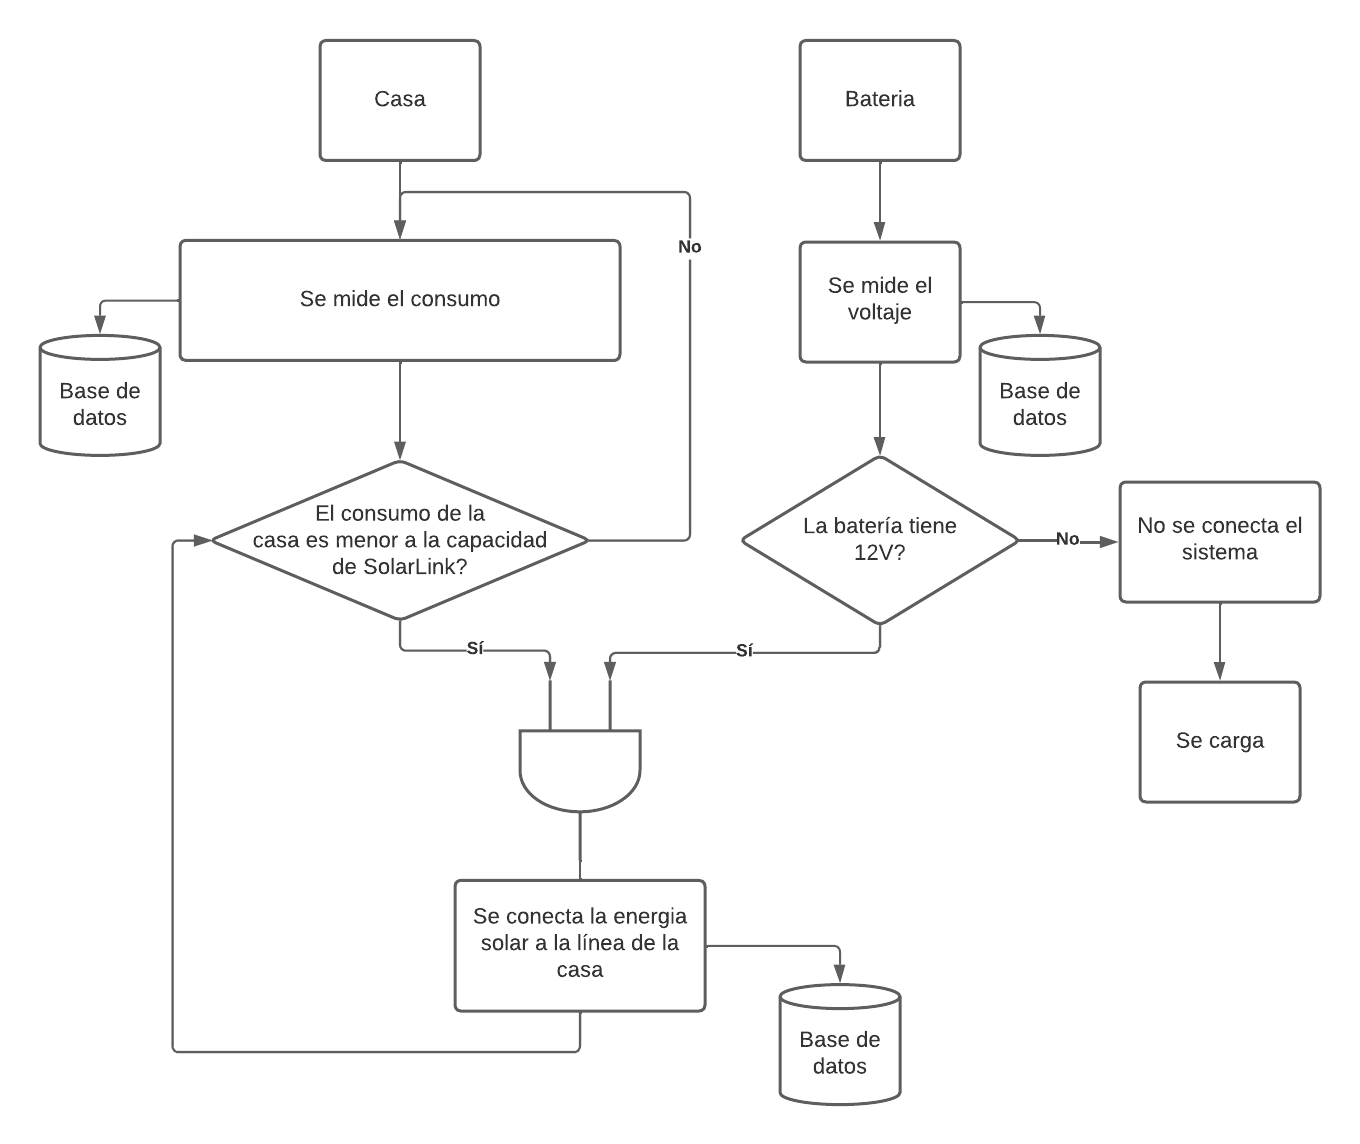
\includegraphics[width=1\linewidth]{analisis-tecnico/Diagrama de flujo SolarLink.png}
    \caption{Diagrama de flujo de Solar Link.}
    \label{fig:enter-label}
\end{figure}

\begin{figure}[H]
    \centering
    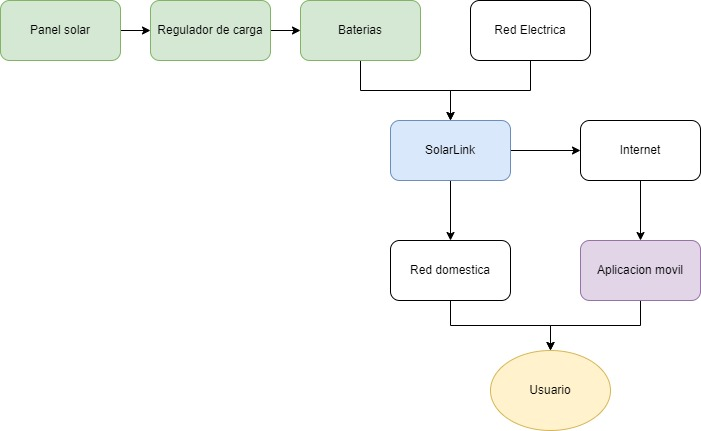
\includegraphics[width=1\linewidth]{analisis-tecnico/Diagrama SolarLink.jpg}
    \caption{Diagrama en bloque del sistema Solar Link.}
    \label{fig:flujo-solarlink}
\end{figure}

\begin{figure}[H]
    \centering
    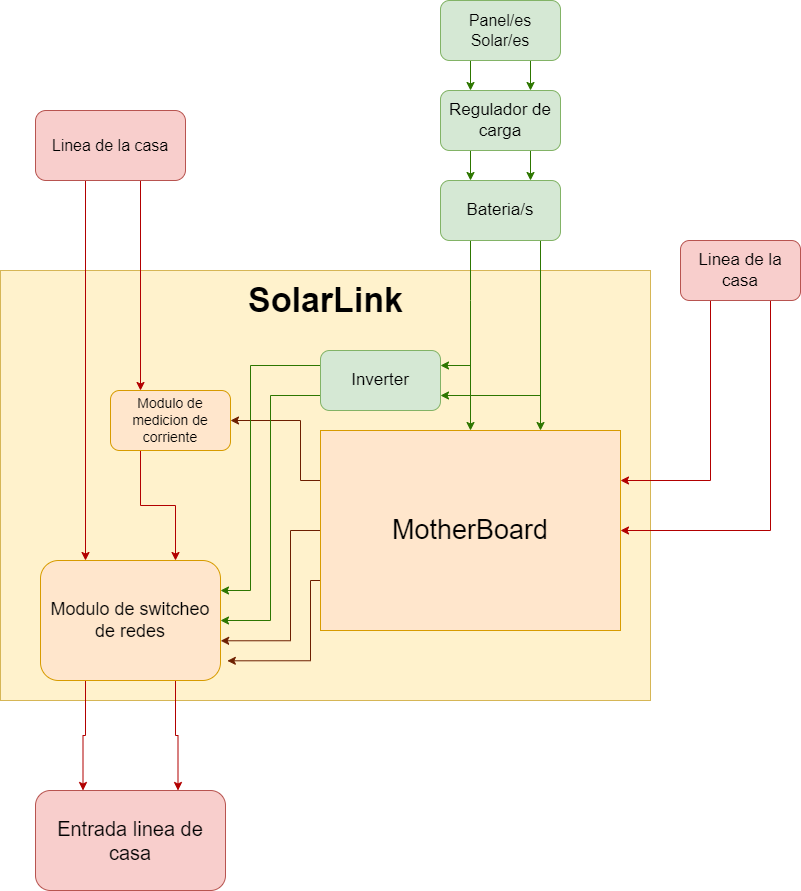
\includegraphics[width=1\linewidth]{analisis-tecnico/Diagrama en bloques.png}
    \caption{Diagrama en bloque del módulo Solar Link.}
    \label{fig:bloque2-solarlink}
\end{figure}

\begin{figure}[H]
    \centering
    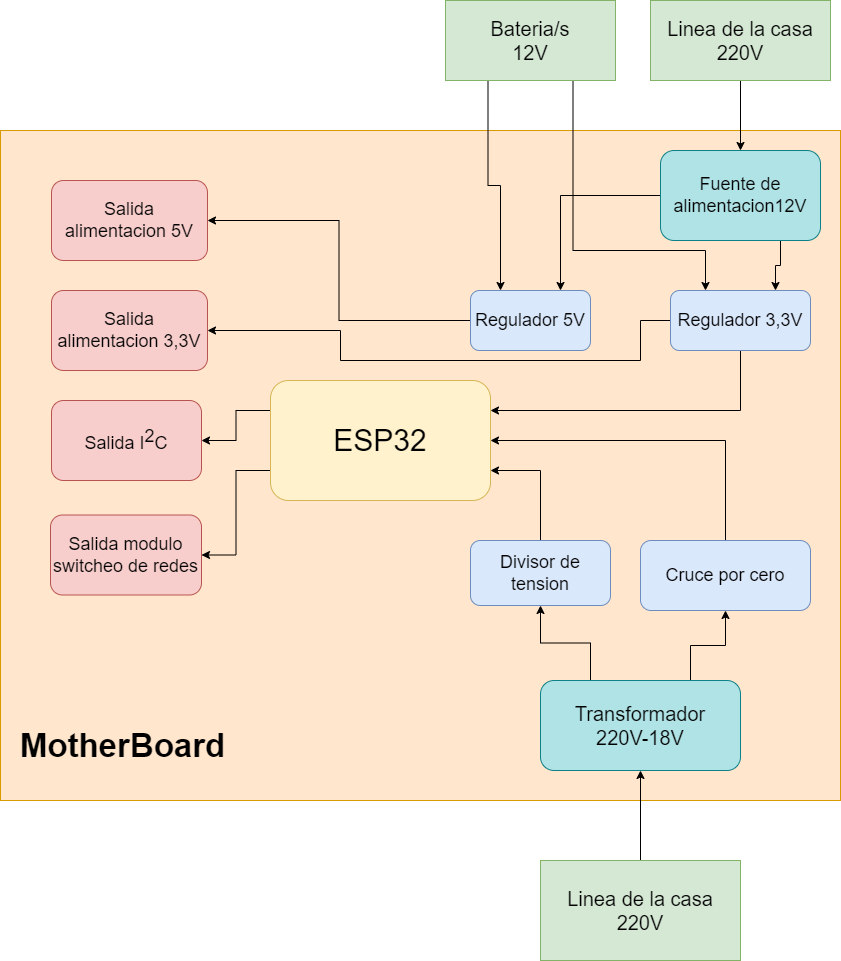
\includegraphics[width=1\linewidth]{analisis-tecnico/Diagrama en bloques mother.png}
    \caption{Diagrama en bloques de la motherboard.}
    \label{fig:diagrama en bloque mother}
\end{figure}

\subsection{Diagramas del cargador MPPT de 3 etapas}

\begin{figure}[H]
    \centering
    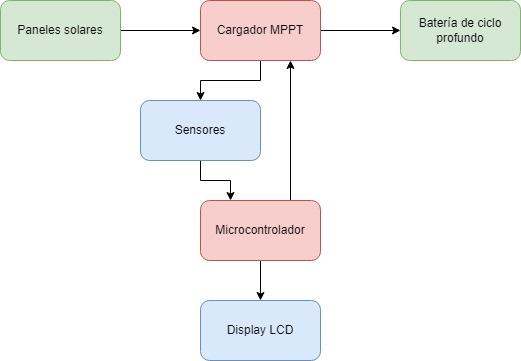
\includegraphics[width=1\linewidth]{analisis-tecnico/Diagrama en bloque MPPT.jpg}
    \caption{Diagrama en bloque del cargador MPPT.}
    \label{fig:diagrama bloque mppt}
\end{figure}

\begin{figure}[H]
    \centering
    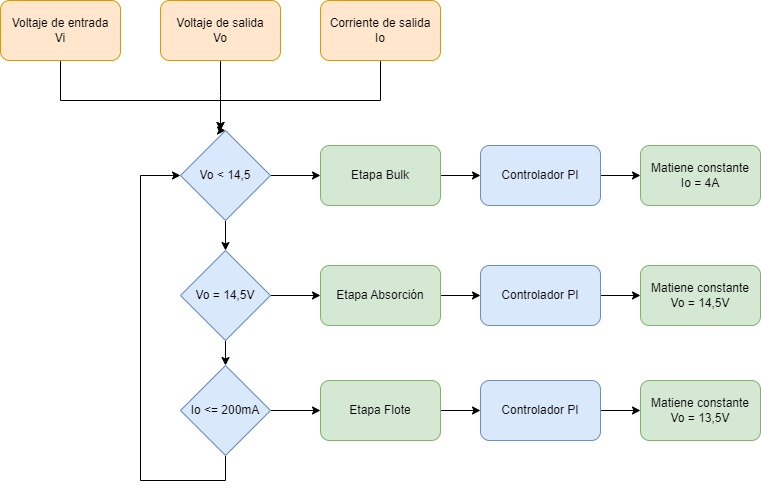
\includegraphics[width=1\linewidth]{analisis-tecnico/Diagrama de flujo MPPT.jpg}
    \caption{Diagrama de flujo del cargador MPPT.}
    \label{fig:diagrama bloque mppt}
\end{figure}